\documentclass[runningheads]{llncs}
\usepackage[ruled]{algorithm2e}
\usepackage{amsfonts}
\usepackage{amsmath}
\usepackage{bm}
\usepackage{booktabs}
\usepackage{color}
\usepackage[compress]{cite}
\usepackage{graphicx}
\usepackage{hyperref}
\usepackage{physics}

\renewcommand\UrlFont{\color{blue}\rmfamily}
\SetKwInput{KwHyperparameters}{Hyperparameters}
\DeclareMathOperator{\sgn}{sgn}
\DeclareMathOperator*{\argmax}{arg\,max}

\begin{document}

\title{
    Multiclass Classification with Pegasos
}
\author{Gabriele Cerizza}
\authorrunning{G. Cerizza}

\institute{Università degli Studi di Milano\\
\email{gabriele.cerizza@studenti.unimi.it}\\
\url{https://github.com/gabrielecerizza/smml}}

\maketitle

\section*{Introduction}
\label{sec:introduction}

In this report we detail the results of our experiments on the Pegasos algorithm~\cite{shalev-pegasos-2011} over a multiclass classification task, pursuant to the project specifications set out for the Statistical Methods for Machine Learning course of the Università degli Studi di Milano\footnote{\url{https://cesa-bianchi.di.unimi.it/MSA/index\_21-22.html}}. 

In Section~\ref{sec:dataset} we illustrate the dataset used in the experiments. In Section~\ref{sec:algorithm} we briefly describe the algorithm and its implementation. In Section~\ref{sec:experiments} we show the results of our experiments and provide comments thereon. Finally, Section~\ref{sec:conclusions} contains our concluding remarks. 

\section{Dataset}
\label{sec:dataset}

Our analysis was carried out on the USPS dataset\footnote{\url{https://www.kaggle.com/datasets/bistaumanga/usps-dataset}}, comprising 9298 $16 \times 16$ grayscale images. These images depict handwritten digits ranging from 0 to 9. A sample of these digits can be seen in Figure~\ref{fig:dataset:digits}. The classes do not present severe imbalance issues, as shown in Figure~\ref{fig:dataset:class_counts}.

To gauge the complexity of multiclass classification on this dataset, we performed dimensionality reduction by way of the t-distributed Stochastic Neighbor Embedding (t-SNE)~\cite{maaten-2008-tsne} algorithm and projected the instances onto a two-dimensional space. The result is given in Figure~\ref{fig:dataset:tsne}. Within this figure the instances are clustered into ten clearly distinguishable groups, thus suggesting that a satisfying classification can be attained.   

The USPS dataset is made available with predetermined training and test sets. In our experiments, however, we merged these sets and proceeded to form our own training and test sets, as illustrated in Section~\ref{sec:experiments}. 

\begin{figure}
  \center
  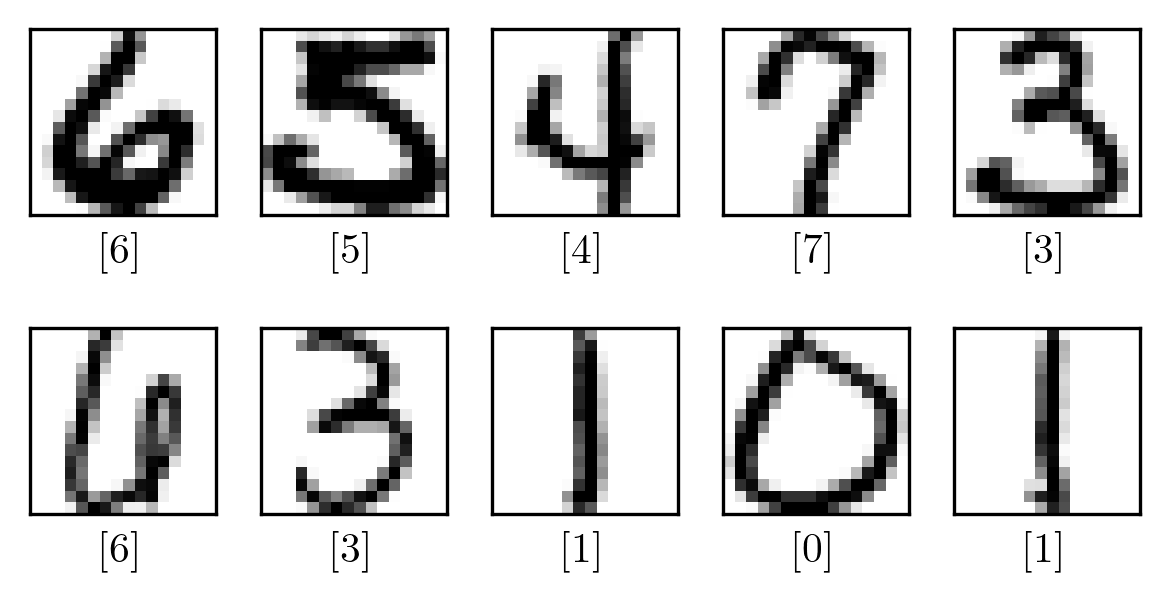
\includegraphics[width=0.7\textwidth]{../img/digits.png}
  \caption{Sample of images from the USPS dataset. The label is indicated below each image.} 
  \label{fig:dataset:digits}
\end{figure}

\begin{figure}
  \center
  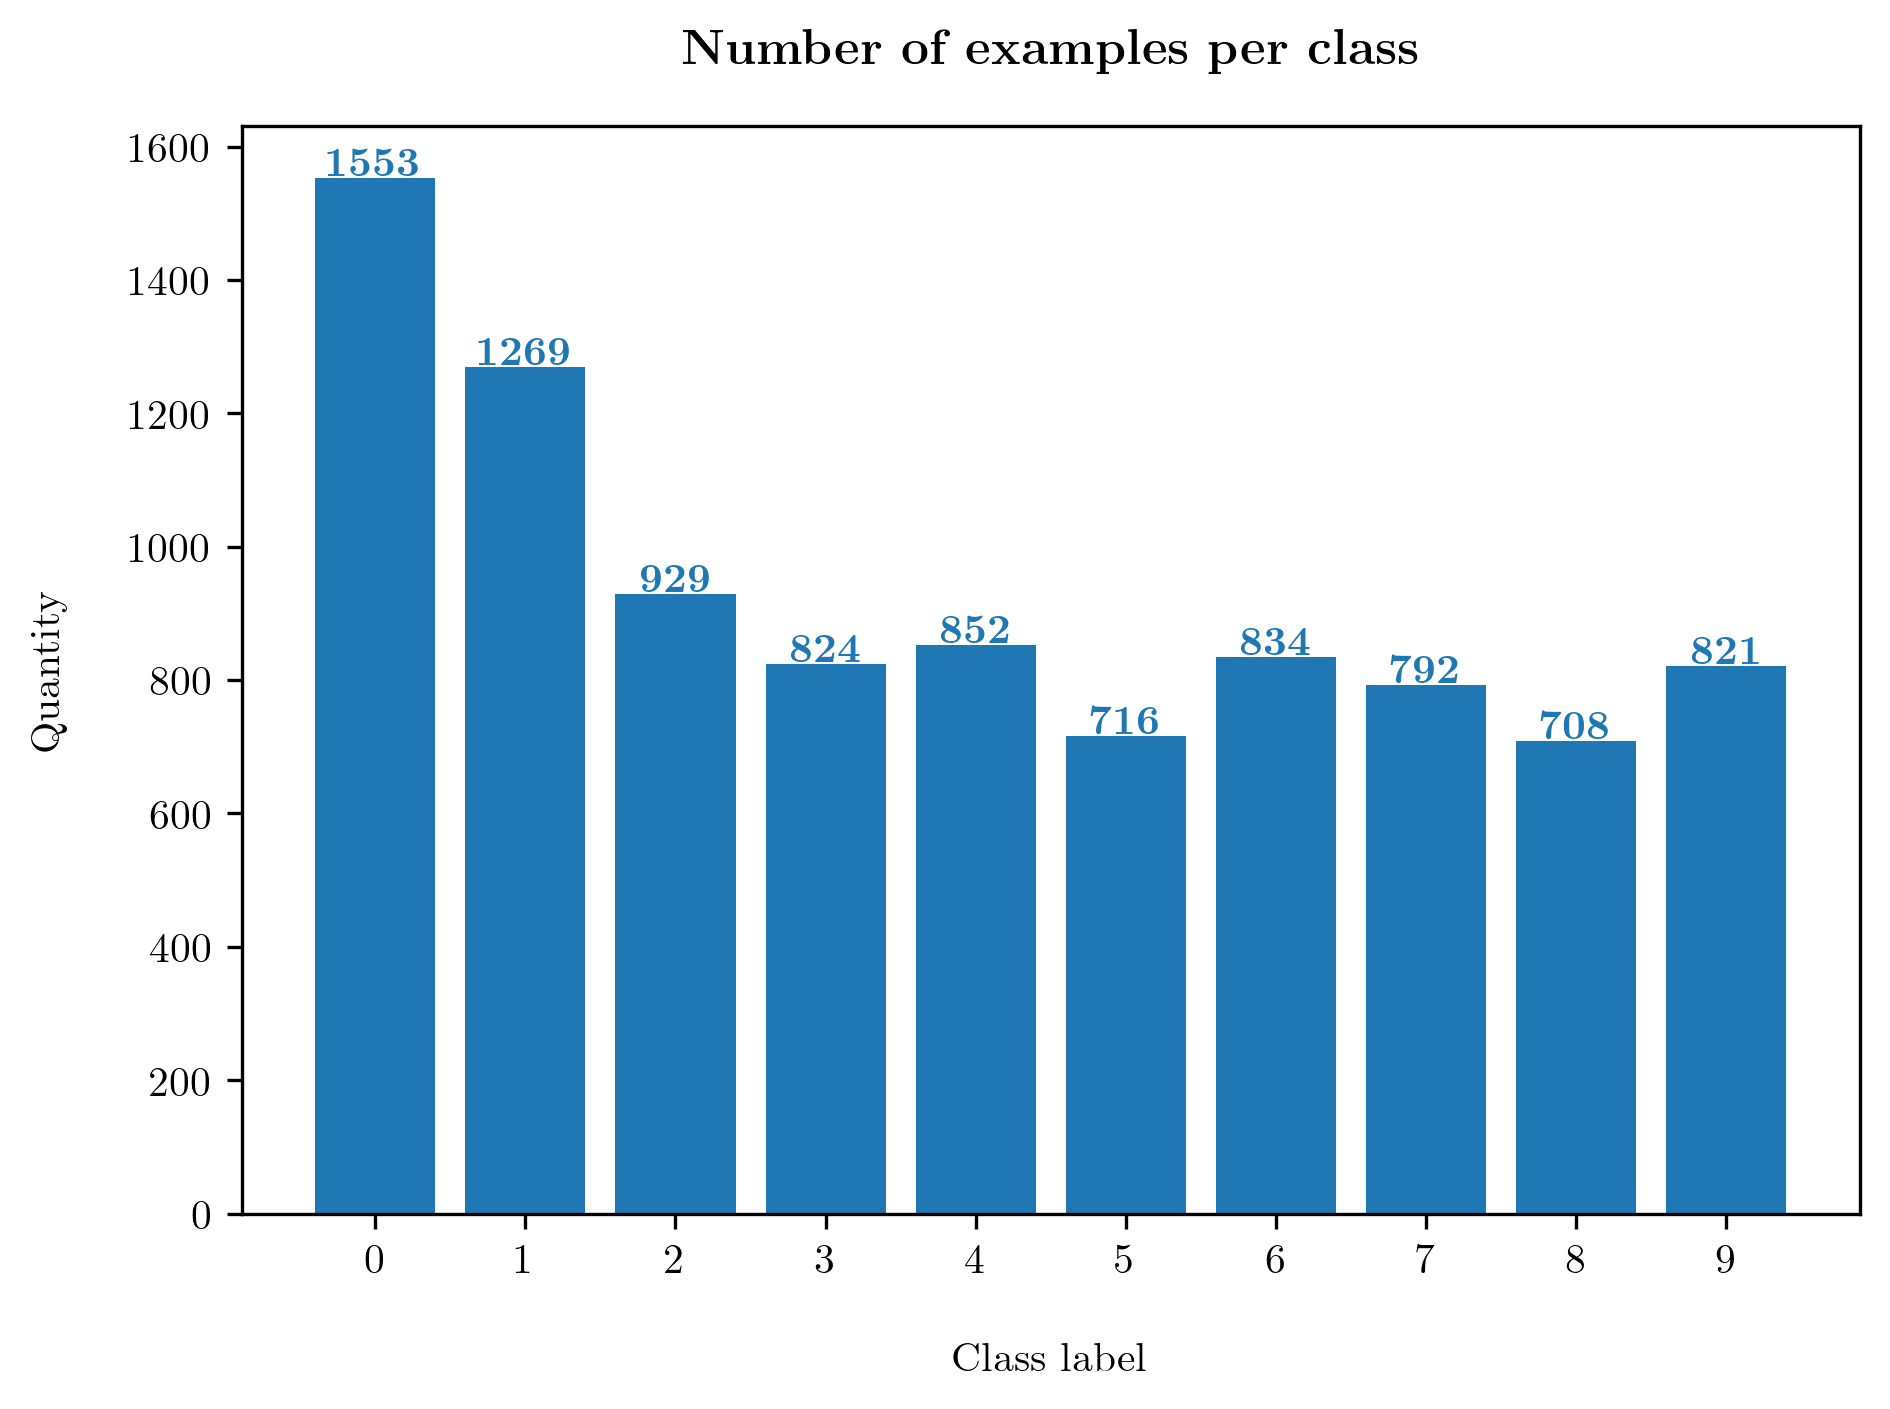
\includegraphics[width=1\textwidth]{../img/class_counts.png}
  \caption{Frequency of the classes in the USPS dataset.} 
  \label{fig:dataset:class_counts}
\end{figure}

\begin{figure}
  \center
  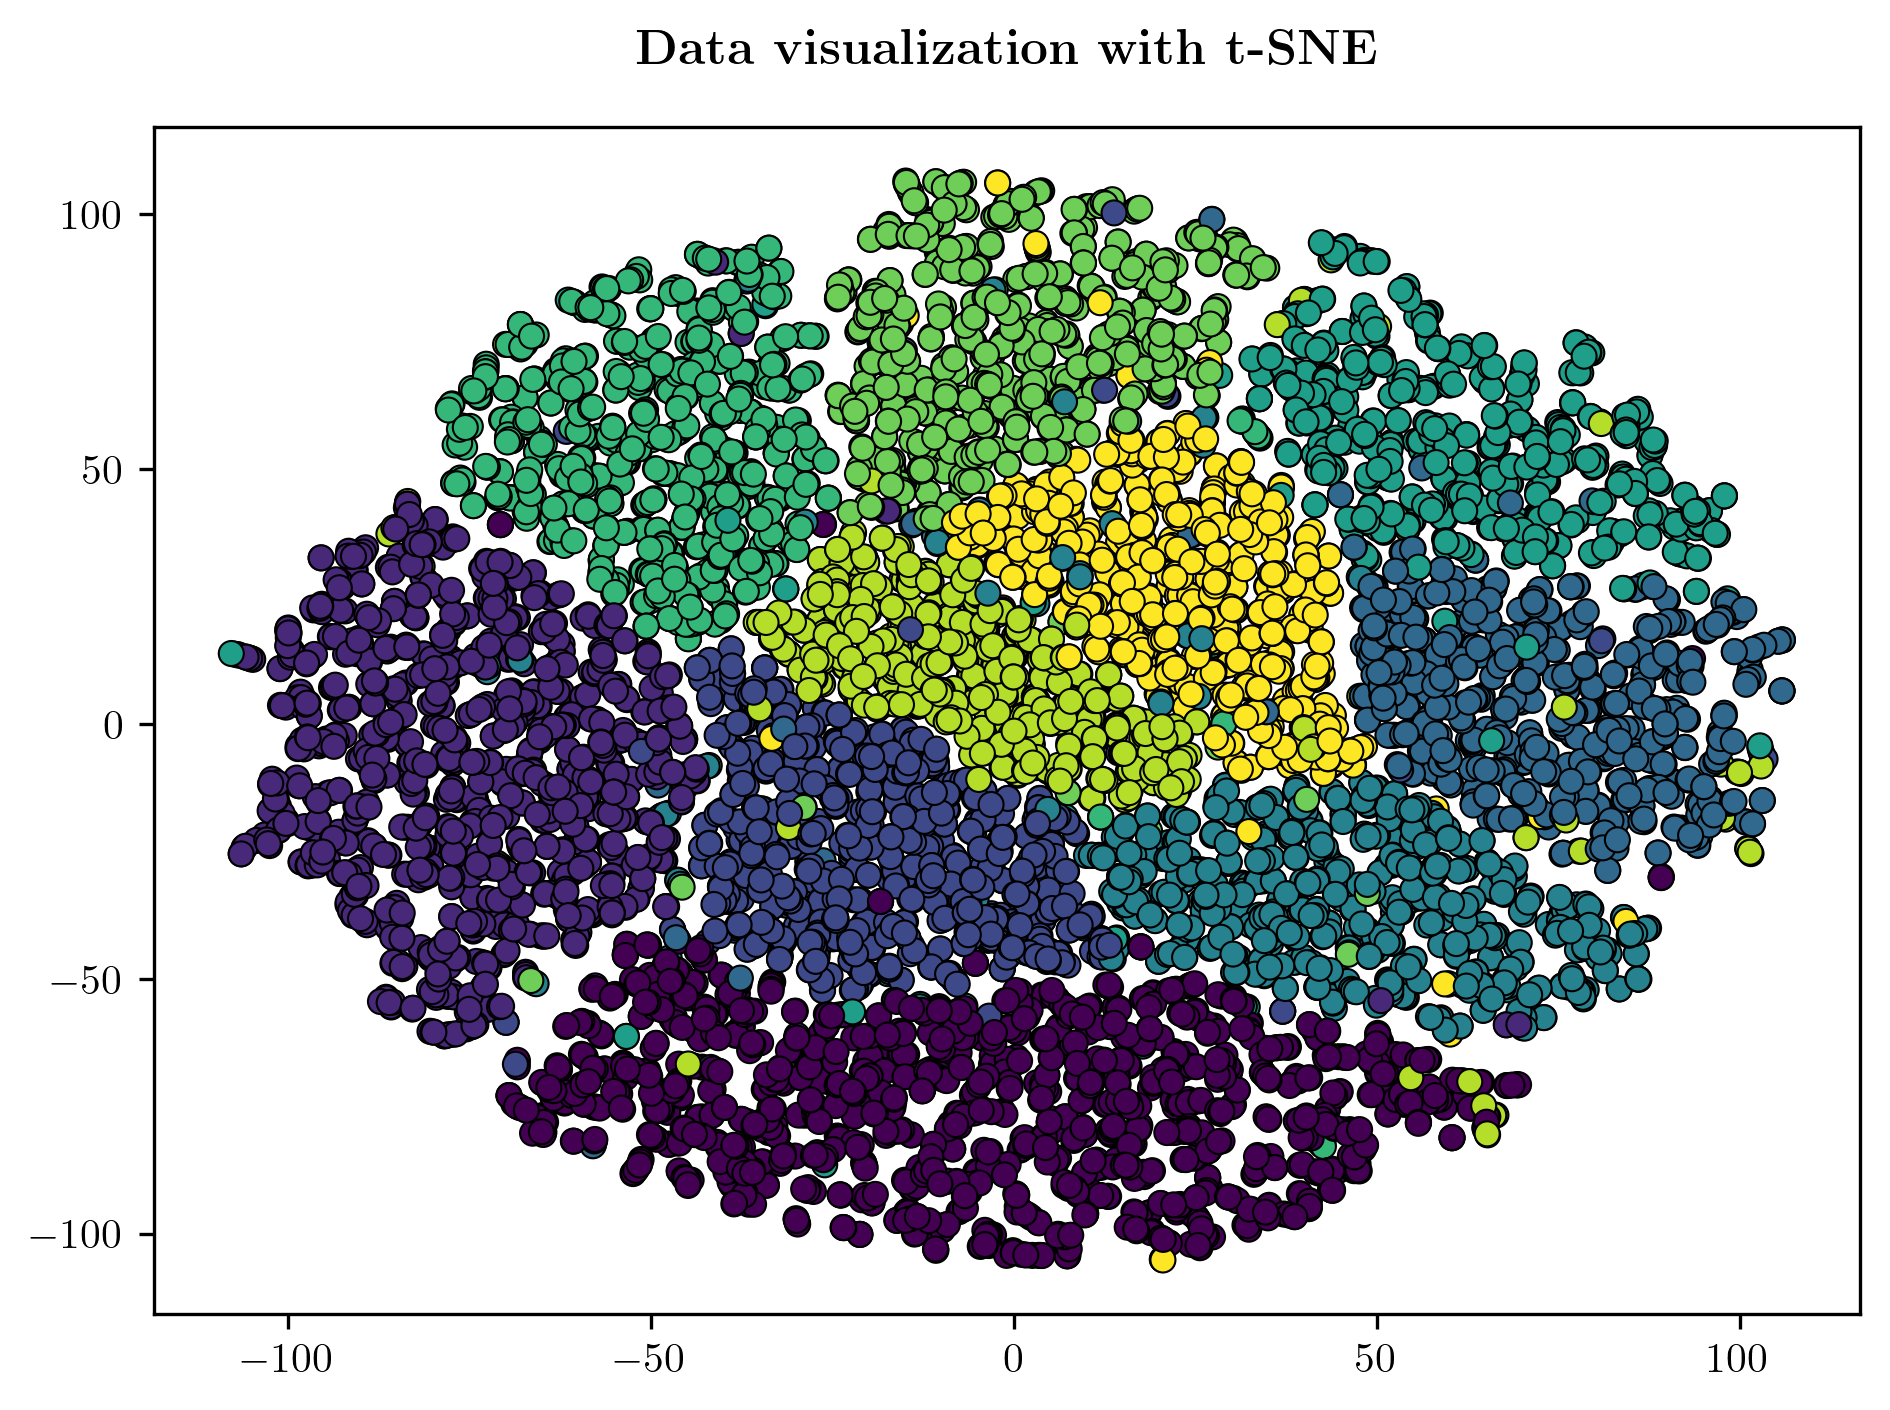
\includegraphics[width=1\textwidth]{../img/tsne.png}
  \caption{Projection of the USPS dataset onto a two-dimensional space using t-SNE.} 
  \label{fig:dataset:tsne}
\end{figure}

\section{Pegasos Algorithm}
\label{sec:algorithm}

In the present section we describe the Pegasos algorithm 

\subsection{Description}
\label{subsec:algorithm:description}

In order to perform the multiclass classification task, we employed the Pegasos algorithm~\cite{shalev-pegasos-2011}. This algorithm was introduced to solve the Support Vector Machine (SVM)~\cite{vapnik-1999-statistical-learning} convex optimization problem for binary classification, which can be formalized as follows. 

Let $S = \{(\bm{x}_1,y_1),\dots,(\bm{x}_m,y_m)\}$ be a training set with $\bm{x}_t \in \mathbb{R}^d \; \forall t=1,\dots,m$ and $y \in \{-1, 1\}$; and let $\phi_K : \mathbb{R}^d \to \mathcal{H}_K$ be a function such that $\text{dim}(\mathcal{H}_K) \gg d$ and $\langle \cdot , \cdot \rangle_K$ is the inner product in $\mathcal{H}_K$. The optimization problem aims to find the maximum margin separating hyperplane in $\mathcal{H}_K$, which separates the examples according to their labels and maximizes the distance between the hyperplane and the closest example. This results in the following quadratic programming problem: 
\begin{alignat}{3}
  &\min_{g \in \mathcal{H}_K, \bm{\xi} \in \mathbb{R}^m} & \quad & \frac{\lambda}{2} \norm{g}_K^2 + \frac{1}{m}\sum_{t=1}^{m} \xi_t \, , \label{eqn:svm}\\
  &\text{subject to}  &       & y_t \langle g, \phi_K(\bm{x}_t) \rangle_K \geq 1 - \xi_t &\qquad& t = 1,\dots,m \, , \notag\\
  &                   &       & \xi_t \geq 0  &\qquad& t = 1,\dots,m \, , \notag
\end{alignat}
where $\lambda$ is a regularization coefficient dictating the relative importance of the two terms in the objective function; and $\xi_t$ are slack variables that allow, but penalize, examples lying on the wrong side of the hyperplane.

This formulation can be turned into the following unconstrained optimization problem:
\begin{equation}
  \min_{g \in \mathcal{H}_K} \quad \frac{\lambda}{2} \norm{g}_K^2 + \frac{1}{m}\sum_{t=1}^{m} h_t(g) \, , \label{eqn:svm_unconstrained}
\end{equation}
where $h_t(g) = [1 - y_t\langle g, \phi_K(\bm{x}_t) \rangle_K]_+$ is the hinge loss.

Pegasos solves this optimization problem using a stochastic gradient descent approach. The algorithm performs $T$ iterations, each of which consists in drawing a training example uniformly at random and updating $g$ through a gradient step. In particular, at iteration $t$ Pegasos computes
\begin{equation}
  g_{t+1} = \frac{1}{\lambda t} \sum_{r = 1}^{t} \mathbb{I}\{h_{s_r}(g_r) > 0\} y_{s_r} K(\bm{x}_{s_r}, \cdot) \, , \label{eqn:pegasos:g}
\end{equation}
where $\mathbb{I}$ is the indicator function, $s_r$ is the index of the example randomly drawn at iteration $r$, and $K : \mathbb{R}^d \times \mathbb{R}^d \to \mathbb{R}$ is a kernel function such that $K(\bm{x},\bm{x}^\prime) = \langle \phi_K(\bm{x}), \phi_K(\bm{x}^\prime) \rangle_K$.

Note that $g_{t+1}$ is a function, not a vector. Indeed, the dot in $K(\bm{x}_{s_r}, \cdot)$ stands for a missing argument, corresponding to the example on which the function is evaluated. Therefore, unlike vectors, $g_{t+1}$ cannot be stored in memory as is and used to perform inference on new examples, since we first have to evaluate $g_{t+1}$ on them.

In order to simplify the process, it was observed in~\cite{shalev-pegasos-2011} that (\ref{eqn:pegasos:g}) can be rewritten as
\begin{equation}
  g_{t+1} = \frac{1}{\lambda t} \sum_{j = 1}^{m} \bm{\alpha}_{t+1}[j] y_j K(\bm{x}_j, \cdot) \, , \label{eqn:pegasos:g_alpha}
\end{equation}
where $\bm{\alpha}_{t+1} \in \mathbb{R}^m$ is a vector representing how many times each example $\bm{x}_j$ in the training set has been drawn and resulted in a non-zero loss, that is
\[
  \bm{\alpha}_{t+1}[j] = 	\lvert \{r \leq t : s_r = j \land y_j\langle g_r, \phi_K(\bm{x}_j) \rangle_K < 1 \} \rvert \, .
\]
The vector $\bm{\alpha}_{t+1}$ can be kept in memory and used to quickly evaluate $g_{t+1}$ on new examples during both training and test. Algorithm~\ref{alg:pegasos} shows the pseudocode for the kernelized Pegasos algorithm using the abovementioned approach.    

\begin{algorithm}
  \DontPrintSemicolon
  \caption{Pegasos algorithm in a kernel space}\label{alg:pegasos}
  \KwHyperparameters{$T$, $\lambda > 0$}
  \KwData{Training set $S = \{(\bm{x}_1,y_1),\dots,(\bm{x}_m,y_m)\}$}
  $\bm{\alpha}_1 \gets (0,\dots,0)$\;
  \For{$t=1$ \KwTo $T$}{   
    Choose $s_r \in \{0,\dots, \lvert S \rvert\}$ uniformly at random \;
    \If{$\frac{1}{\lambda t} \sum_{j = 1}^{m} \bm{\alpha}_{t + 1}[j] y_j K(\bm{x}_j, \bm{x}_{s_r}) < 1$}{
      $\bm{\alpha}_{t+1}[s_r] = \bm{\alpha}_{t}[s_r] + 1$\;
    }
  }
  \Return $\bm{\alpha}_{T+1}$
\end{algorithm}

Once the vector $\bm{\alpha}_{T+1}$ has been obtained, the label of a new example $\bm{x}$ can be predicted by computing
\begin{equation}
  \hat{y} = \sgn \left( \sum_{j = 1}^{m} \bm{\alpha}_{T+1}[j] y_j K(\bm{x}_j, \bm{x}) \right) \, .
\end{equation}
It is not necessary to multiply the sum by $\frac{1}{\lambda T}$, since scaling does not affect the sign.

So far we illustrated the Pegasos algorithm for binary classification. In order to handle multiclass classification, we prepare a different binary classifier for each class. These binary classifiers are trained using labels encoded as $1$ for the examples belonging to the class of the classifier, and encoded as $-1$ for the examples belonging to all the other classes. 

Finally, to determine the class of a new example $\bm{x}$, we first compute
\begin{equation}
  h_i = \sum_{j = 1}^{m} \bm{\alpha}_{T+1}[j] y_j K(\bm{x}_j, \bm{x}) \,
  \label{eqn:pegasos:h_i}
\end{equation}
for each classifier $c_i$, and then predict with
\[
  \hat{y} = \argmax_i {h_i} \, .
\]
Also in this case scaling $h_i$ is unnecessary, given that $\frac{1}{\lambda T}$ is always positive and therefore does not change the order of the $h_i$ values.

What sets the Pegasos algorithm apart from other algorithms developed to solve the SVM problem is its ability to converge to a solution that differs from the optimal solution by less than $\epsilon$ in $O(\frac{1}{\lambda \epsilon})$ iterations with high probability with respect to the random draws of the training examples. In other terms, the convergence rate does not depend on the size of the training set, but only on the number of iterations, making Pegasos a suitable algorithm to perform classification over large datasets.  

\subsection{Kernel functions}
\label{subsec:algorithm:kernel}

The Pegasos algorithm is agnostic of the kernel function. In our experiments, we employed two kernel functions: the Gaussian kernel and the polynomial kernel. The Gaussian kernel is defined as
\[
  K(\bm{x},\bm{x}^\prime) = \exp(-\frac{1}{2 \gamma}\norm{\bm{x} - \bm{x}^\prime}^2) \, ,
\]
with $\gamma > 0$. The polynomial kernel is defined as
\[
  K(\bm{x},\bm{x}^\prime) = (1 + \bm{x}^\top \bm{x}^\prime)^n \, ,  
\]
where $n \in \mathbb{N}$ is the degree of the polynomial. 

\subsection{Implementation}
\label{subsec:algorithm:implementation}

In this section we expound on two implementation details employed to improve the runtime of the algorithm.

\subsubsection{Kernel matrix.} In order to perform multiclass classification, we trained multiple classifiers, each slated to run the Pegasos algorithm over the same training set. Within this framework, the kernel function between two given examples may be computed multiple times, resulting in redundant computations.

Moreover, at each iteration the Pegasos algorithm computes the kernel function between a randomly drawn training example and all the other training examples. Drawing the same example multiple times results in further redundant computations.

Redundant computations adversely affect the runtime of the algorithm and should therefore be avoided. To this effect, we opted to compute ahead of time the kernel matrix $K$, such that
\[
  K_{i,j} = K(\bm{x}_i, \bm{x}_j) \quad \forall i,j=1,\dots,m \, .
\]
This matrix was then dispatched to each classifier and used in place of the kernel function evaluation.

The drawback of the kernel matrix lies in its memory footprint. However, given the size of the USPS dataset, such a matrix would require in the worst case $\frac{9298 \times 9298 \times 32}{2^3 \times 10^9} \approx 0.34$ gigabytes of memory, which in modern machines constitutes a negligible amount.  

\subsubsection{Vectorization.} The summations within the Pegasos algorithm can be vectorized, thus allowing to exploit the highly optimized array operations made available by math libraries.

In particular, the condition of the \texttt{if} statement within Algorithm~\ref{alg:pegasos} can be rewritten as
\[
  \frac{1}{\lambda t} (\bm{\alpha}_t \odot y)^\top K_{s_r} < 1 \, ,
\]
where $\odot$ is the Hadamard product and $K$ is the kernel matrix between the training examples. Whereas the formula for $h_i$ in (\ref{eqn:pegasos:h_i}) can be rewritten as
\[
  \bm{h}_i = (\bm{\alpha}_{T+1} \odot y)^\top K^\prime \, ,
\]
where $K^\prime$ is the kernel matrix between the training examples and the test examples and $\bm{h}_i$ is the vector containing the predictions for all test examples returned by classifier $c_i$.

Also the computation of the kernel matrices can be vectorized. In the case of the polynomial kernel, the vectorization is trivial.

alpha is a vector, bold

This is exacerbated




Remove tags for equations unless needed

Under scrutiny

\section{Experiments}
\label{sec:experiments}

The experiments were run on a machine with 16 GB of
RAM and a CPU Intel(R) Core(TM) i7-9700K 3.60GHz with 8 cores.



\section{Conclusions}
\label{sec:conclusions}

\section*{Statement}
\textit{I/We declare that this material, which I/We now submit for assessment, is entirely my/our own work and has not been taken from the work of others, save and to the extent that such work has been cited and acknowledged within the text of my/our work. I/We understand that plagiarism, collusion, and copying are grave and serious offences in the university and accept the penalties that would be imposed should I engage in plagiarism, collusion or copying. This assignment, or any part of it, has not been previously submitted by me/us or any other person for assessment on this or any other course of study.}


\bibliographystyle{splncs04}
\bibliography{bibtex_entries}

\end{document}